%*******************************************************************
%  Crypto World Bank — Pre-Thesis 2 Project Demonstration Poster
%  Layout follows academy "Good" examples (clean 3-column, navy brand
%  bars, readable figures). Avoids "Bad" patterns: dense walls of text,
%  overlapping columns, gradient backgrounds, tiny unreadable charts.
%  Content source: v40 thesis (prose condensed for poster distance).
%*******************************************************************
\documentclass[10pt]{article}

\usepackage[a1paper,landscape,margin=12mm,bottom=22mm]{geometry}
\usepackage[T1]{fontenc}
\usepackage[utf8]{inputenc}
\usepackage{lmodern}
\usepackage{graphicx}
\usepackage{xcolor}
\usepackage{booktabs}
\usepackage{array}
\usepackage{enumitem}
\usepackage{tabularx}
\usepackage{colortbl}
\usepackage{amsmath}
\usepackage{tikz}
\IfFileExists{qrcode.sty}{\usepackage{qrcode}}{}
\usepackage{hyperref}
\hypersetup{colorlinks=true,urlcolor=NavyBrand,linkcolor=NavyBrand}

\definecolor{NavyBrand}{HTML}{0B1F3A}
\definecolor{AccentGold}{HTML}{C9A227}
\definecolor{SoftGray}{HTML}{F4F6F8}
\definecolor{Muted}{HTML}{4A5568}
\definecolor{TableHead}{HTML}{E8EEF5}

\pagestyle{empty}
\setlength{\parindent}{0pt}
\setlength{\parskip}{0.35em}
\setlist[itemize]{leftmargin=1.1em,itemsep=0.15em,topsep=0.2em,parsep=0pt}
\setlist[enumerate]{leftmargin=1.2em,itemsep=0.15em,topsep=0.2em,parsep=0pt}

\newcommand{\PosterSection}[1]{%
  \vspace{0.55em}%
  {\Large\bfseries\color{NavyBrand}\MakeUppercase{#1}\par}%
  {\color{AccentGold}\rule{\linewidth}{2.2pt}\par}%
  \vspace{0.35em}%
}

\newcommand{\PosterFig}[2]{%
  \begin{center}
    \includegraphics[width=\linewidth,height=#1,keepaspectratio]{#2}%
  \end{center}%
}

\newcommand{\FigCap}[1]{%
  {\footnotesize\color{Muted}\textit{#1}\par}%
  \vspace{0.2em}%
}

\begin{document}

% ===================== HEADER =====================
\noindent
\begin{tikzpicture}[remember picture,overlay]
  \fill[NavyBrand] (current page.north west) rectangle ([yshift=-5.0cm]current page.north east);
  \fill[AccentGold] ([yshift=-5.0cm]current page.north west) rectangle ([yshift=-5.15cm]current page.north east);
\end{tikzpicture}

\vspace*{-0.2cm}
\noindent
\begin{minipage}[c]{0.12\textwidth}
  \centering
  \colorbox{white}{
\includegraphics[width=0.92\linewidth]{../images/bracu_logo_12-0-2022.pdf}}
\end{minipage}%
\hfill
\begin{minipage}[c]{0.72\textwidth}
  \centering
  {\fontsize{30}{34}\selectfont\bfseries\color{white} Decentralized Crypto World Bank\par}
  \vspace{0.2em}
  {\fontsize{14}{17}\selectfont\color{white!92} A Blockchain-Based Hierarchical Banking Platform with AI-Enhanced Security\par}
  \vspace{0.4em}
  {\fontsize{12}{15}\selectfont\color{white}
    Md.\ Bokhtiar Rahman Juboraz (20301138) \quad\textbullet\quad
    Md.\ Mahir Ahnaf Ahmed (20301083)\par}
  \vspace{0.12em}
  {\fontsize{10.5}{13}\selectfont\color{AccentGold}
    Thesis ID: P26101123 \quad\textbullet\quad
    Department of Computer Science and Engineering \quad\textbullet\quad
    BRAC University\par}
\end{minipage}%
\hfill
\begin{minipage}[c]{0.12\textwidth}
  \centering
  \ifdefined\qrcode
    \colorbox{white}{\qrcode[height=2.4cm]{https://github.com/Yuvraajrahman/Cryto-World-Bank}}\\[0.25em]
    {\scriptsize\color{white}\bfseries Scan repo}
  \else
    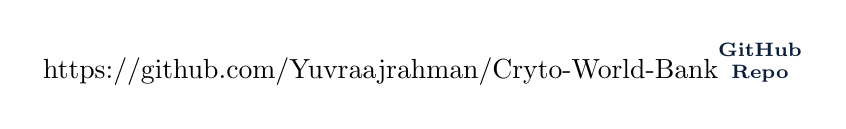
\begin{tikzpicture}
      \node[draw=white,line width=1.2pt,inner sep=5pt,fill=white,rounded corners=2pt] {
        \href{https://github.com/Yuvraajrahman/Cryto-World-Bank}{\scriptsize\bfseries\color{NavyBrand}\shortstack{GitHub\\Repo}}
      };
    \end{tikzpicture}
  \fi
\end{minipage}

\vspace{1.35cm}

% ===================== THREE COLUMNS =====================
\noindent
\begin{minipage}[t]{0.315\textwidth}
% -------- LEFT --------
\PosterSection{Abstract}
{\small
Modern institutional banking is layered for governance, yet capital flows remain opaque and slow.
\textit{Crypto World Bank} bridges that hierarchy with programmable DeFi: a four-tier on-chain lending platform
(World Bank $\to$ National $\to$ Local $\to$ Client) with reserve enforcement, multi-entity products,
oracle-mediated ML risk support, and an optional conversational agent.
The goal is a sustainable, auditable prototype that shows hierarchical institutional finance can run on an EVM ledger.
\par\vspace{0.2em}
{\footnotesize\textbf{Keywords:} Hierarchical DeFi, Smart Contracts, Reserve Management, Explainable AI, Group Lending}
}

\PosterSection{Problem \& Motivation}
{\small
Development-finance corridors still face \$45 avg.\ cross-border cost and 2--5 day settlement;
1.4B adults remain unbanked and MSMEs face a \$4.5T financing gap.
Flat DeFi (Aave/Compound) automates pools but ignores institutional hierarchy, inter-tier capital, and local-bank retail paths.
}

{\small\textbf{Structural gaps addressed}}
\begin{itemize}
\item Opaque reserves and tiered decision trails
\item Idle correspondent capital \& slow settlement
\item No unified on-chain credit passport across tiers
\item No programmable solidarity / group credit
\item No explainable ML support for human approvers
\end{itemize}

\PosterSection{Objectives}
\begin{enumerate}[label=\textbf{O\arabic*.},leftmargin=1.6em]
\item{\small Four-tier EVM lending architecture + testnet path (Phases I--IV)}
\item{\small Banking suite: deposits, savings, solidarity group lending}
\item{\small Off-chain ML fraud analytics + optional MCP agent}
\item{\small On-chain limits, installments, role-based access}
\item{\small Deploy/evaluate on Sepolia / Amoy / zkEVM Cardona}
\item{\small Document governance, security, and sandbox rollout}
\end{enumerate}

\PosterSection{Methodology}
{\small
Agile four-phase plan ($\approx$16 weeks). This pre-thesis focuses on architecture, contracts, schema, and ML benchmarks;
Phase~II demonstrates the loan cycle; Phase~III oracle + scoring; Phase~IV evaluation.
\par\vspace{0.25em}
\textbf{Stack:} Solidity \textbullet\ React \textbullet\ Express/FastAPI \textbullet\ PostgreSQL \textbullet\ scikit-learn
\par
\textbf{Settlement:} single-chain (Sepolia/Amoy); multi-chain deferred for bridge risk.
}

\end{minipage}%
\hfill
\begin{minipage}[t]{0.315\textwidth}
% -------- MIDDLE --------
\PosterSection{System Overview}
\PosterFig{7.2cm}{../images/architecture_diagram_fixed.pdf}
\FigCap{Figure 1. Four-tier Crypto World Bank system overview.}

\PosterSection{Cross-Tier Capital Flows}
\PosterFig{7.0cm}{../images/fund_flow_diagram_v2.pdf}
\FigCap{Figure 2. Downward allocation, peer lending, upward deposits, and syndication.}

\PosterSection{Architecture Layers}
\PosterFig{5.4cm}{../images/fig-three-layer-arch.pdf}
\FigCap{Figure 3. Presentation, application/oracle, and on-chain contract layers.}

\end{minipage}%
\hfill
\begin{minipage}[t]{0.315\textwidth}
% -------- RIGHT --------
\PosterSection{Demonstration Results}
{\small
\textbf{ML fraud support} (BCCC-DeFiFraudTrans-2025 subsample, 50k txs, $\approx$8.7\% fraud; 21 features; wallet-safe split).
Human approvers remain in the loop; scores commit on-chain via commit--reveal.
}

\vspace{0.3em}
\renewcommand{\arraystretch}{1.25}
{\footnotesize
\begin{tabular}{@{}lcccc@{}}
\rowcolor{TableHead}
\textbf{Split} & \textbf{Prec.} & \textbf{Rec.} & \textbf{F1} & \textbf{AUC} \\
\midrule
Held-out test & 0.874 & 0.908 & \textbf{0.891} & 0.991 \\
\end{tabular}
\par\vspace{0.15em}
TN\,=\,4{,}621; FP\,=\,60; FN\,=\,42; TP\,=\,417 \quad($n_{\text{test}}=5{,}140$)
}

\vspace{0.35em}
\PosterFig{4.6cm}{../images/fig-ml-metrics-bars.pdf}
\FigCap{Figure 4. Precision / Recall / F1 / ROC-AUC on held-out wallets.}

\vspace{0.2em}
\PosterFig{4.2cm}{../images/fig-ml-confusion-matrix.pdf}
\FigCap{Figure 5. Confusion matrix for the stacked RF + Isolation Forest pipeline.}

\PosterSection{Key Design Choices}
\begin{itemize}
\item{\small Stablecoin-first retail path (avoid ETH liability volatility)}
\item{\small L2 / testnet gas target $\approx$\$0.011 per loan lifecycle}
\item{\small Off-chain RF+IF+SHAP; on-chain gates only}
\item{\small Optional local agent (MCP banking tools) for demo UX}
\end{itemize}

\PosterSection{Conclusion}
{\small
CWB shows hierarchical development-finance flows can be encoded as auditable smart-contract state with
explainable ML assisting---not replacing---credit judgment. Next: Phase~II--IV MVT loan E2E on testnet,
oracle latency, and CWB-specific model retrain as live traffic arrives.
}

\PosterSection{Selected References}
{\scriptsize
\begin{enumerate}[label={[\arabic*]},leftmargin=1.4em,itemsep=0.12em]
\item Werner et al. 2022. SoK: Decentralized Finance (DeFi). arXiv:2101.08778.
\item Palaiokrassas et al. 2024. Leveraging ML for Multichain DeFi Fraud Detection. IEEE ICBC.
\item World Bank. 2021. Global Findex Database 2021.
\item IFC. 2017. MSME Finance Gap.
\item Liu, Ting \& Zhou. 2008. Isolation Forest. IEEE ICDM.
\item Atzei, Bartoletti \& Cimoli. 2017. Attacks on Ethereum Smart Contracts. POST.
\end{enumerate}
}

\end{minipage}

% ===================== FOOTER =====================
\begin{tikzpicture}[remember picture,overlay]
  \fill[NavyBrand] (current page.south west) rectangle ([yshift=1.55cm]current page.south east);
  \fill[AccentGold] ([yshift=1.55cm]current page.south west) rectangle ([yshift=1.70cm]current page.south east);
  \node[anchor=west,text=white,font=\large\bfseries] at ([xshift=1.2cm,yshift=0.75cm]current page.south west)
    {Pre-thesis 2: Project Demonstration Poster};
  \node[anchor=east,text=white,font=\large] at ([xshift=-1.2cm,yshift=0.75cm]current page.south east)
    {BRAC University CSE \textbullet\ Open source: github.com/Yuvraajrahman/Cryto-World-Bank};
\end{tikzpicture}

\end{document}
